% Created by tikzDevice version 0.12
% !TEX encoding = UTF-8 Unicode
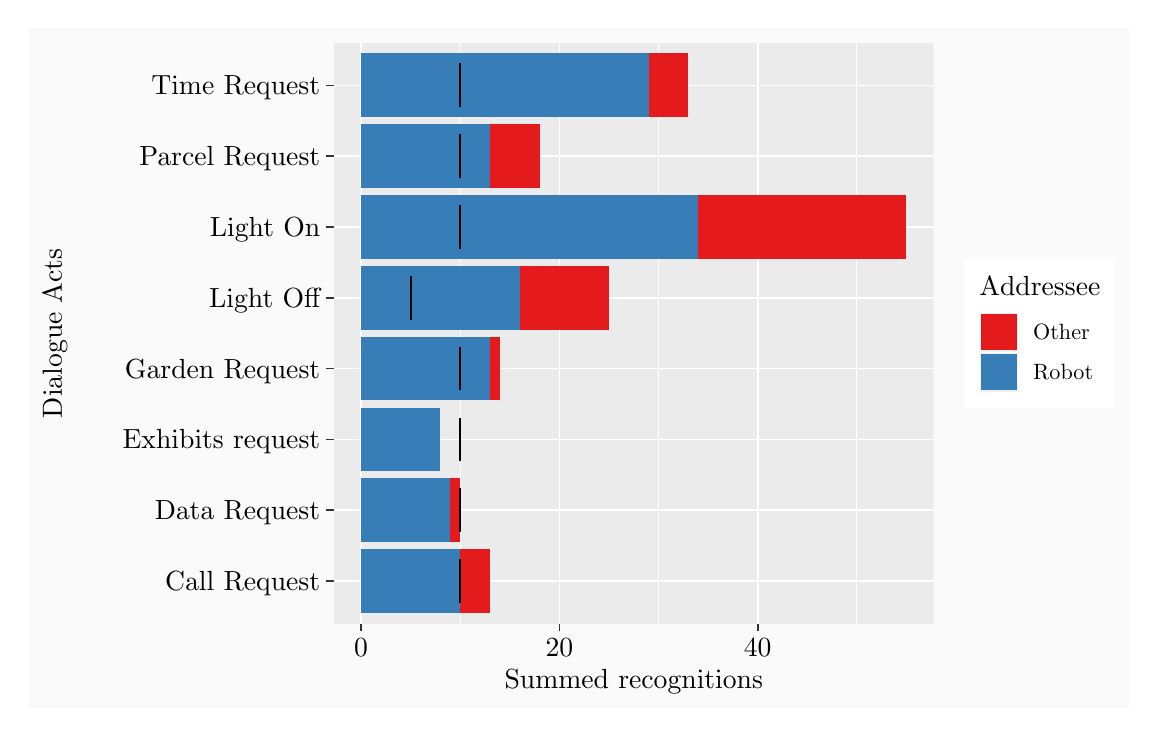
\begin{tikzpicture}[x=1pt,y=1pt]
\definecolor{fillColor}{RGB}{255,255,255}
\path[use as bounding box,fill=fillColor,fill opacity=0.00] (0,0) rectangle (398.34,246.17);
\begin{scope}
\path[clip] (  0.00,  0.00) rectangle (398.34,246.17);
\definecolor{drawColor}{RGB}{255,255,255}
\definecolor{fillColor}{gray}{0.98}

\path[draw=drawColor,line width= 0.6pt,line join=round,line cap=round,fill=fillColor] (  0.00,  0.00) rectangle (398.34,246.17);
\end{scope}
\begin{scope}
\path[clip] (110.65, 30.86) rectangle (327.38,240.67);
\definecolor{fillColor}{gray}{0.92}

\path[fill=fillColor] (110.65, 30.86) rectangle (327.38,240.67);
\definecolor{drawColor}{RGB}{255,255,255}

\path[draw=drawColor,line width= 0.3pt,line join=round] (156.33, 30.86) --
	(156.33,240.67);

\path[draw=drawColor,line width= 0.3pt,line join=round] (227.97, 30.86) --
	(227.97,240.67);

\path[draw=drawColor,line width= 0.3pt,line join=round] (299.61, 30.86) --
	(299.61,240.67);

\path[draw=drawColor,line width= 0.6pt,line join=round] (110.65, 46.21) --
	(327.38, 46.21);

\path[draw=drawColor,line width= 0.6pt,line join=round] (110.65, 71.80) --
	(327.38, 71.80);

\path[draw=drawColor,line width= 0.6pt,line join=round] (110.65, 97.39) --
	(327.38, 97.39);

\path[draw=drawColor,line width= 0.6pt,line join=round] (110.65,122.97) --
	(327.38,122.97);

\path[draw=drawColor,line width= 0.6pt,line join=round] (110.65,148.56) --
	(327.38,148.56);

\path[draw=drawColor,line width= 0.6pt,line join=round] (110.65,174.15) --
	(327.38,174.15);

\path[draw=drawColor,line width= 0.6pt,line join=round] (110.65,199.73) --
	(327.38,199.73);

\path[draw=drawColor,line width= 0.6pt,line join=round] (110.65,225.32) --
	(327.38,225.32);

\path[draw=drawColor,line width= 0.6pt,line join=round] (120.50, 30.86) --
	(120.50,240.67);

\path[draw=drawColor,line width= 0.6pt,line join=round] (192.15, 30.86) --
	(192.15,240.67);

\path[draw=drawColor,line width= 0.6pt,line join=round] (263.79, 30.86) --
	(263.79,240.67);
\definecolor{fillColor}{RGB}{55,126,184}

\path[fill=fillColor] (120.50, 34.70) rectangle (156.33, 57.73);
\definecolor{fillColor}{RGB}{228,26,28}

\path[fill=fillColor] (156.33, 34.70) rectangle (167.07, 57.73);
\definecolor{fillColor}{RGB}{55,126,184}

\path[fill=fillColor] (120.50, 60.29) rectangle (152.74, 83.32);
\definecolor{fillColor}{RGB}{228,26,28}

\path[fill=fillColor] (152.74, 60.29) rectangle (156.33, 83.32);
\definecolor{fillColor}{RGB}{55,126,184}

\path[fill=fillColor] (120.50, 85.87) rectangle (149.16,108.90);

\path[fill=fillColor] (120.50,111.46) rectangle (167.07,134.49);
\definecolor{fillColor}{RGB}{228,26,28}

\path[fill=fillColor] (167.07,111.46) rectangle (170.65,134.49);
\definecolor{fillColor}{RGB}{55,126,184}

\path[fill=fillColor] (120.50,137.05) rectangle (177.82,160.08);
\definecolor{fillColor}{RGB}{228,26,28}

\path[fill=fillColor] (177.82,137.05) rectangle (210.06,160.08);
\definecolor{fillColor}{RGB}{55,126,184}

\path[fill=fillColor] (120.50,162.63) rectangle (242.30,185.66);
\definecolor{fillColor}{RGB}{228,26,28}

\path[fill=fillColor] (242.30,162.63) rectangle (317.53,185.66);
\definecolor{fillColor}{RGB}{55,126,184}

\path[fill=fillColor] (120.50,188.22) rectangle (167.07,211.25);
\definecolor{fillColor}{RGB}{228,26,28}

\path[fill=fillColor] (167.07,188.22) rectangle (184.98,211.25);
\definecolor{fillColor}{RGB}{55,126,184}

\path[fill=fillColor] (120.50,213.81) rectangle (224.39,236.84);
\definecolor{fillColor}{RGB}{228,26,28}

\path[fill=fillColor] (224.39,213.81) rectangle (238.72,236.84);
\definecolor{drawColor}{RGB}{0,0,0}

\path[draw=drawColor,line width= 0.6pt,line join=round] (156.33, 38.31) --
	(156.33, 54.12);

\path[draw=drawColor,line width= 0.6pt,line join=round] (156.33, 46.21) --
	(156.33, 46.21);

\path[draw=drawColor,line width= 0.6pt,line join=round] (156.33, 38.31) --
	(156.33, 54.12);

\path[draw=drawColor,line width= 0.6pt,line join=round] (156.33, 38.31) --
	(156.33, 54.12);

\path[draw=drawColor,line width= 0.6pt,line join=round] (156.33, 46.21) --
	(156.33, 46.21);

\path[draw=drawColor,line width= 0.6pt,line join=round] (156.33, 38.31) --
	(156.33, 54.12);

\path[draw=drawColor,line width= 0.6pt,line join=round] (156.33, 63.89) --
	(156.33, 79.71);

\path[draw=drawColor,line width= 0.6pt,line join=round] (156.33, 71.80) --
	(156.33, 71.80);

\path[draw=drawColor,line width= 0.6pt,line join=round] (156.33, 63.89) --
	(156.33, 79.71);

\path[draw=drawColor,line width= 0.6pt,line join=round] (156.33, 63.89) --
	(156.33, 79.71);

\path[draw=drawColor,line width= 0.6pt,line join=round] (156.33, 71.80) --
	(156.33, 71.80);

\path[draw=drawColor,line width= 0.6pt,line join=round] (156.33, 63.89) --
	(156.33, 79.71);

\path[draw=drawColor,line width= 0.6pt,line join=round] (156.33, 89.48) --
	(156.33,105.29);

\path[draw=drawColor,line width= 0.6pt,line join=round] (156.33, 97.39) --
	(156.33, 97.39);

\path[draw=drawColor,line width= 0.6pt,line join=round] (156.33, 89.48) --
	(156.33,105.29);

\path[draw=drawColor,line width= 0.6pt,line join=round] (156.33,115.07) --
	(156.33,130.88);

\path[draw=drawColor,line width= 0.6pt,line join=round] (156.33,122.97) --
	(156.33,122.97);

\path[draw=drawColor,line width= 0.6pt,line join=round] (156.33,115.07) --
	(156.33,130.88);

\path[draw=drawColor,line width= 0.6pt,line join=round] (156.33,115.07) --
	(156.33,130.88);

\path[draw=drawColor,line width= 0.6pt,line join=round] (156.33,122.97) --
	(156.33,122.97);

\path[draw=drawColor,line width= 0.6pt,line join=round] (156.33,115.07) --
	(156.33,130.88);

\path[draw=drawColor,line width= 0.6pt,line join=round] (138.41,140.65) --
	(138.41,156.47);

\path[draw=drawColor,line width= 0.6pt,line join=round] (138.41,148.56) --
	(138.41,148.56);

\path[draw=drawColor,line width= 0.6pt,line join=round] (138.41,140.65) --
	(138.41,156.47);

\path[draw=drawColor,line width= 0.6pt,line join=round] (138.41,140.65) --
	(138.41,156.47);

\path[draw=drawColor,line width= 0.6pt,line join=round] (138.41,148.56) --
	(138.41,148.56);

\path[draw=drawColor,line width= 0.6pt,line join=round] (138.41,140.65) --
	(138.41,156.47);

\path[draw=drawColor,line width= 0.6pt,line join=round] (156.33,166.24) --
	(156.33,182.05);

\path[draw=drawColor,line width= 0.6pt,line join=round] (156.33,174.15) --
	(156.33,174.15);

\path[draw=drawColor,line width= 0.6pt,line join=round] (156.33,166.24) --
	(156.33,182.05);

\path[draw=drawColor,line width= 0.6pt,line join=round] (156.33,166.24) --
	(156.33,182.05);

\path[draw=drawColor,line width= 0.6pt,line join=round] (156.33,174.15) --
	(156.33,174.15);

\path[draw=drawColor,line width= 0.6pt,line join=round] (156.33,166.24) --
	(156.33,182.05);

\path[draw=drawColor,line width= 0.6pt,line join=round] (156.33,191.83) --
	(156.33,207.64);

\path[draw=drawColor,line width= 0.6pt,line join=round] (156.33,199.73) --
	(156.33,199.73);

\path[draw=drawColor,line width= 0.6pt,line join=round] (156.33,191.83) --
	(156.33,207.64);

\path[draw=drawColor,line width= 0.6pt,line join=round] (156.33,191.83) --
	(156.33,207.64);

\path[draw=drawColor,line width= 0.6pt,line join=round] (156.33,199.73) --
	(156.33,199.73);

\path[draw=drawColor,line width= 0.6pt,line join=round] (156.33,191.83) --
	(156.33,207.64);

\path[draw=drawColor,line width= 0.6pt,line join=round] (156.33,217.41) --
	(156.33,233.23);

\path[draw=drawColor,line width= 0.6pt,line join=round] (156.33,225.32) --
	(156.33,225.32);

\path[draw=drawColor,line width= 0.6pt,line join=round] (156.33,217.41) --
	(156.33,233.23);

\path[draw=drawColor,line width= 0.6pt,line join=round] (156.33,217.41) --
	(156.33,233.23);

\path[draw=drawColor,line width= 0.6pt,line join=round] (156.33,225.32) --
	(156.33,225.32);

\path[draw=drawColor,line width= 0.6pt,line join=round] (156.33,217.41) --
	(156.33,233.23);
\end{scope}
\begin{scope}
\path[clip] (  0.00,  0.00) rectangle (398.34,246.17);
\definecolor{drawColor}{RGB}{0,0,0}

\node[text=drawColor,anchor=base east,inner sep=0pt, outer sep=0pt, scale=  1.00] at (105.70, 42.77) {Call Request};

\node[text=drawColor,anchor=base east,inner sep=0pt, outer sep=0pt, scale=  1.00] at (105.70, 68.36) {Data Request};

\node[text=drawColor,anchor=base east,inner sep=0pt, outer sep=0pt, scale=  1.00] at (105.70, 93.94) {Exhibits request};

\node[text=drawColor,anchor=base east,inner sep=0pt, outer sep=0pt, scale=  1.00] at (105.70,119.53) {Garden Request};

\node[text=drawColor,anchor=base east,inner sep=0pt, outer sep=0pt, scale=  1.00] at (105.70,145.12) {Light Off};

\node[text=drawColor,anchor=base east,inner sep=0pt, outer sep=0pt, scale=  1.00] at (105.70,170.70) {Light On};

\node[text=drawColor,anchor=base east,inner sep=0pt, outer sep=0pt, scale=  1.00] at (105.70,196.29) {Parcel Request};

\node[text=drawColor,anchor=base east,inner sep=0pt, outer sep=0pt, scale=  1.00] at (105.70,221.88) {Time Request};
\end{scope}
\begin{scope}
\path[clip] (  0.00,  0.00) rectangle (398.34,246.17);
\definecolor{drawColor}{gray}{0.20}

\path[draw=drawColor,line width= 0.6pt,line join=round] (107.90, 46.21) --
	(110.65, 46.21);

\path[draw=drawColor,line width= 0.6pt,line join=round] (107.90, 71.80) --
	(110.65, 71.80);

\path[draw=drawColor,line width= 0.6pt,line join=round] (107.90, 97.39) --
	(110.65, 97.39);

\path[draw=drawColor,line width= 0.6pt,line join=round] (107.90,122.97) --
	(110.65,122.97);

\path[draw=drawColor,line width= 0.6pt,line join=round] (107.90,148.56) --
	(110.65,148.56);

\path[draw=drawColor,line width= 0.6pt,line join=round] (107.90,174.15) --
	(110.65,174.15);

\path[draw=drawColor,line width= 0.6pt,line join=round] (107.90,199.73) --
	(110.65,199.73);

\path[draw=drawColor,line width= 0.6pt,line join=round] (107.90,225.32) --
	(110.65,225.32);
\end{scope}
\begin{scope}
\path[clip] (  0.00,  0.00) rectangle (398.34,246.17);
\definecolor{drawColor}{gray}{0.20}

\path[draw=drawColor,line width= 0.6pt,line join=round] (120.50, 28.11) --
	(120.50, 30.86);

\path[draw=drawColor,line width= 0.6pt,line join=round] (192.15, 28.11) --
	(192.15, 30.86);

\path[draw=drawColor,line width= 0.6pt,line join=round] (263.79, 28.11) --
	(263.79, 30.86);
\end{scope}
\begin{scope}
\path[clip] (  0.00,  0.00) rectangle (398.34,246.17);
\definecolor{drawColor}{RGB}{0,0,0}

\node[text=drawColor,anchor=base,inner sep=0pt, outer sep=0pt, scale=  1.00] at (120.50, 19.03) {0};

\node[text=drawColor,anchor=base,inner sep=0pt, outer sep=0pt, scale=  1.00] at (192.15, 19.03) {20};

\node[text=drawColor,anchor=base,inner sep=0pt, outer sep=0pt, scale=  1.00] at (263.79, 19.03) {40};
\end{scope}
\begin{scope}
\path[clip] (  0.00,  0.00) rectangle (398.34,246.17);
\definecolor{drawColor}{RGB}{0,0,0}

\node[text=drawColor,anchor=base,inner sep=0pt, outer sep=0pt, scale=  1.00] at (219.01,  7.44) {Summed recognitions};
\end{scope}
\begin{scope}
\path[clip] (  0.00,  0.00) rectangle (398.34,246.17);
\definecolor{drawColor}{RGB}{0,0,0}

\node[text=drawColor,rotate= 90.00,anchor=base,inner sep=0pt, outer sep=0pt, scale=  1.00] at ( 12.39,135.77) {Dialogue Acts};
\end{scope}
\begin{scope}
\path[clip] (  0.00,  0.00) rectangle (398.34,246.17);
\definecolor{fillColor}{RGB}{255,255,255}

\path[fill=fillColor] (338.38,108.90) rectangle (392.84,162.64);
\end{scope}
\begin{scope}
\path[clip] (  0.00,  0.00) rectangle (398.34,246.17);
\definecolor{drawColor}{RGB}{0,0,0}

\node[text=drawColor,anchor=base west,inner sep=0pt, outer sep=0pt, scale=  1.00] at (343.88,149.28) {Addressee};
\end{scope}
\begin{scope}
\path[clip] (  0.00,  0.00) rectangle (398.34,246.17);
\definecolor{drawColor}{RGB}{255,255,255}
\definecolor{fillColor}{gray}{0.95}

\path[draw=drawColor,line width= 0.6pt,line join=round,line cap=round,fill=fillColor] (343.88,128.85) rectangle (358.33,143.31);
\end{scope}
\begin{scope}
\path[clip] (  0.00,  0.00) rectangle (398.34,246.17);
\definecolor{fillColor}{RGB}{228,26,28}

\path[fill=fillColor] (344.59,129.56) rectangle (357.62,142.59);
\end{scope}
\begin{scope}
\path[clip] (  0.00,  0.00) rectangle (398.34,246.17);
\definecolor{drawColor}{RGB}{255,255,255}
\definecolor{fillColor}{gray}{0.95}

\path[draw=drawColor,line width= 0.6pt,line join=round,line cap=round,fill=fillColor] (343.88,114.40) rectangle (358.33,128.85);
\end{scope}
\begin{scope}
\path[clip] (  0.00,  0.00) rectangle (398.34,246.17);
\definecolor{fillColor}{RGB}{55,126,184}

\path[fill=fillColor] (344.59,115.11) rectangle (357.62,128.14);
\end{scope}
\begin{scope}
\path[clip] (  0.00,  0.00) rectangle (398.34,246.17);
\definecolor{drawColor}{RGB}{0,0,0}

\node[text=drawColor,anchor=base west,inner sep=0pt, outer sep=0pt, scale=  0.80] at (363.33,133.32) {Other};
\end{scope}
\begin{scope}
\path[clip] (  0.00,  0.00) rectangle (398.34,246.17);
\definecolor{drawColor}{RGB}{0,0,0}

\node[text=drawColor,anchor=base west,inner sep=0pt, outer sep=0pt, scale=  0.80] at (363.33,118.87) {Robot};
\end{scope}
\end{tikzpicture}
